\CourseSection{Functional Description}\label{sec:functional-description}
\CourseSubsection{System overview}

Since this is a dataset analysis project, the system itself is fairly simple, as shown in Figure~\ref{fig:system}.
GitSkills is distributed as a single SQLite database, with a Parquet copy of each table, and holds four tables: \texttt{artifacts}, \texttt{artifact\_siblings}, \texttt{repos}, and \texttt{mining\_runs}.
The fields we need are queried from these tables into Python, where we rely on common data-analysis libraries: pandas and NumPy for data handling, DuckDB and PyArrow for querying the Parquet files, tiktoken for token counts, textstat for readability formulas, datasketch for MinHash similarity, SciPy and powerlaw for statistics, and Matplotlib for plots.
A pre-processing script first transforms it for the metric scripts and filters out files that are not genuine skills (\texttt{filename}, \texttt{location\_class}, \texttt{frontmatter\_valid}).
The cleaned data then passes to a separate calculation script for each metric, whose methods are described in Section~\ref{sec:design}.
Finally, an output transformation script joins the results into a single metrics file used for analysis, plotting, and validation.
The only input from outside the dataset is a small sample of cloned GitHub repositories used to validate churn.

\begin{figure}[htbp]
\centering
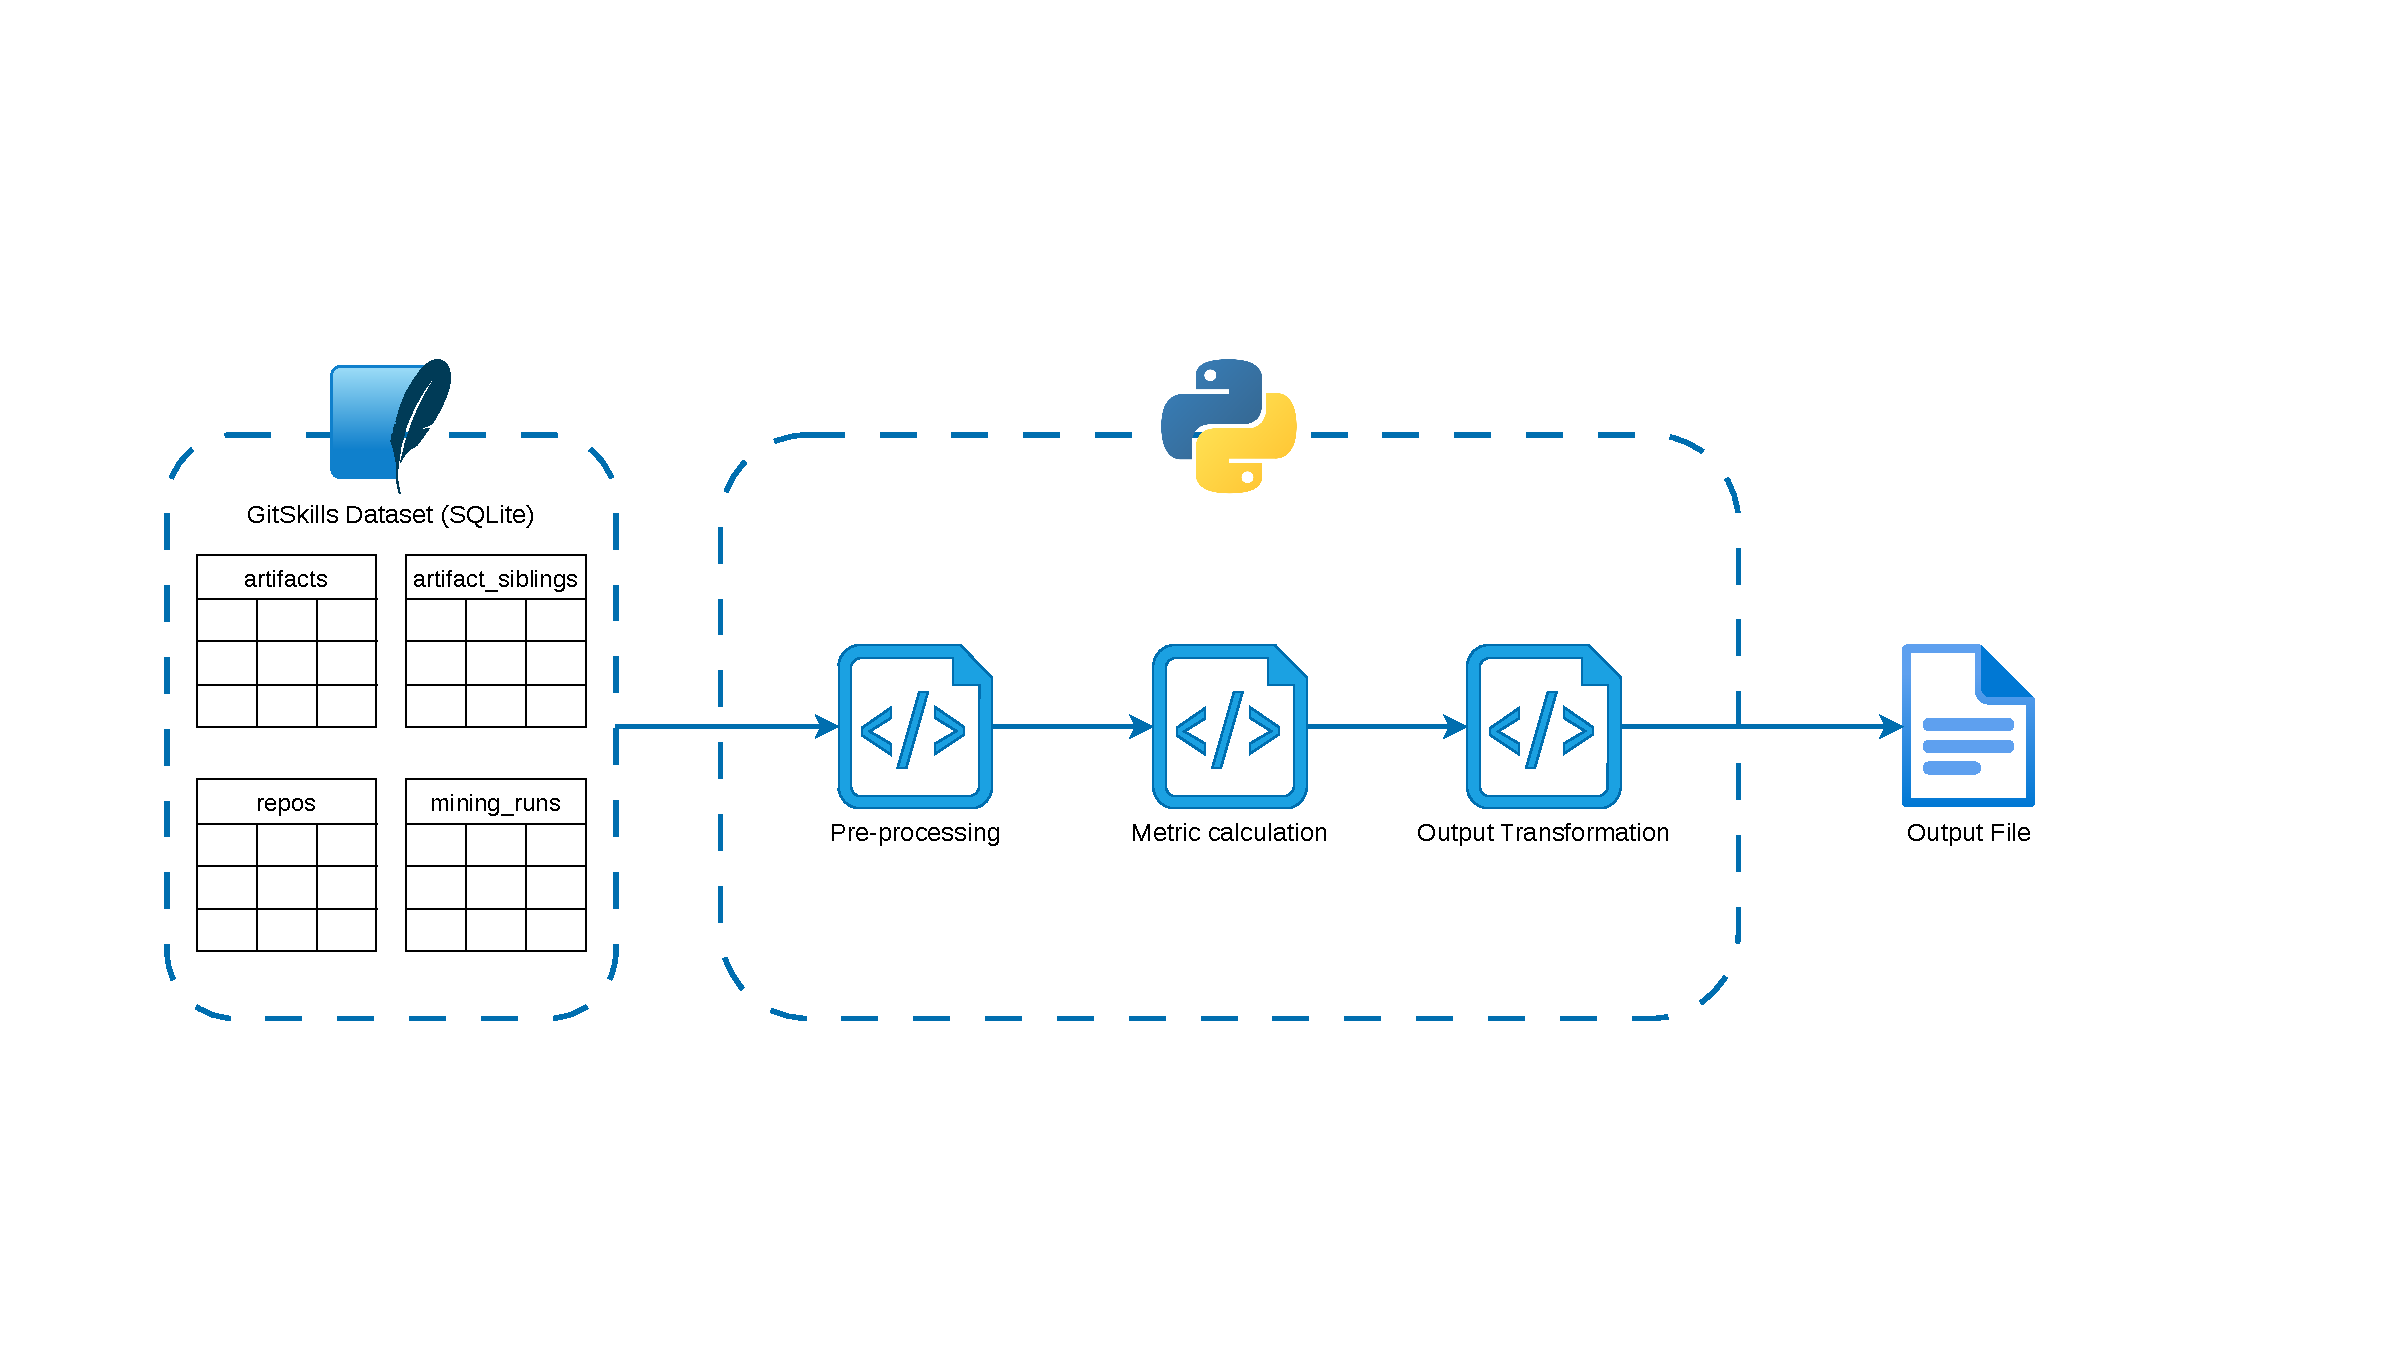
\includegraphics[width=\linewidth]{figures/490CapstoneProposalGeneralFigure1}
\caption{Data flow from the GitSkills tables through the Python pipeline to the final metrics file.}
\label{fig:system}
\end{figure}

\CourseSubsection{Interface and performance specifications}

\begin{singlespace}
\setlength{\LTcapwidth}{\linewidth}
\begin{longtable}{@{}L{0.10\linewidth} L{\dimexpr0.4700000\linewidth-6.0000000\tabcolsep\relax} L{0.22\linewidth} L{0.21\linewidth}@{}}
\caption{Preliminary system specifications.}\label{tab:proposal-specs}\\
\rowcolor{MidGray}
\TableHeader{ID} & \TableHeader{Requirement} & \TableHeader{Target} & \TableHeader{Tolerance} \\
\midrule
\endfirsthead
\rowcolor{MidGray}
\TableHeader{ID} & \TableHeader{Requirement} & \TableHeader{Target} & \TableHeader{Tolerance} \\
\midrule
\endhead
\bottomrule
\endfoot
IF-01 & All four GitSkills tables load into Python with their documented columns & 4 of 4 tables & 0 missing columns \\
\addlinespace[3pt]
IF-02 & Scripts pass data keyed by \texttt{file\_sha}, with no rows lost between stages & 100\% of rows kept & 0 rows \\
\addlinespace[3pt]
IF-03 & Output file holds one row per distinct skill, in Parquet and CSV & 1 row per skill & 0 duplicates \\
\addlinespace[3pt]
PF-01 & Full-dataset run time on one workstation & $\leq$ 24 h & +12 h \\
\addlinespace[3pt]
PF-02 & Peak memory use, kept low through batching & $\leq$ 16 GB & +4 GB \\
\addlinespace[3pt]
PF-03 & Re-running the pipeline reproduces the same metrics & Identical output & 0 differences \\
\addlinespace[3pt]
PF-04 & Precision of cross-copy lineage links on the hand-labelled sample & $\geq$ 0.90 & $-$0.05 \\
\addlinespace[3pt]
PF-05 & Spearman correlation between Flesch--Kincaid grade and the mean human rating on the 100-skill readability sample & $|\rho| \geq$ 0.5 & $-$0.1 \\
\addlinespace[3pt]
PF-06 & Agreement between the two readability raters (Krippendorff's $\alpha$~\cite{krippendorff2004}) & $\geq$ 0.80 & $-$0.13 \\
\end{longtable}
\end{singlespace}

\CourseSubsection{Risks and safety hazards}
The project is purely computational, so it carries no physical, health, or safety hazards.
The main technical risk is the dataset's size (about 44 GB), which is managed by reading the per-table Parquet files in batches rather than loading everything into memory.
Since the data comes from public GitHub repositories with commit authors already anonymized, we will not attempt to identify individuals, and we will respect each repository's license when quoting skill content.
\clearpage
